\documentclass[12pt,twocolumn]{article}
\usepackage{graphicx}
\usepackage{amsmath}
	\DeclareMathOperator{\erf}{erf}
\usepackage{varioref}
\usepackage[colorlinks=false,linkcolor=black,hidelinks]{hyperref}
\usepackage{cleveref}

\title{Error Function}
\author{Jonas Svenstrup Hansen, study no. 201205674}

\begin{document}
\maketitle
In mathematics, the error function (also called the Gauss error function) is a special function (non-elementary) of sigmoid shape that occurs in probability, statistics, and partial differential equations describing diffusion. It is defined as:
\begin{align*}
\erf (x) &= \frac{1}{2\pi}\int_{-x}^{x} e^{-t^2} \, \text{d}t \\
&= \frac{2}{\sqrt{\pi}} \int_0^x e^{-t^2} \, \text{d}t \;.
\end{align*}
In statistics, for nonnegative values of $x$, the error function has the following interpretation: for a random variable $X$ that is normally distributed with mean $0$ and variance $1/2$, $\erf(x)$ describes the probability of $X$ falling in the range $[−x, x]$.
\cite{wiki}

A plot of the error function is shown in \cref{fig:errfunc}.
\begin{figure}
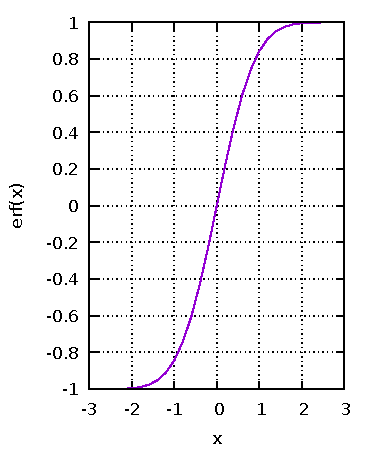
\includegraphics[width=\columnwidth]{plot.pdf}
\caption{The error function.}
\label{fig:errfunc}
\end{figure}


\begin{thebibliography}{1}
	\bibitem{wiki} Wikipedia, the free encyclopedia, \url{https://en.wikipedia.org/wiki/Error_function}
\end{thebibliography}

\end{document}
